%Beamer class
\documentclass{beamer}

\usepackage[czech]{babel}
\usepackage[cp1250]{inputenc}
\usepackage{fontenc}
\usepackage{tgheros}
\usepackage{array}
\usepackage{color}
\usepackage{hyperref}

\usetheme{Antibes}
\usecolortheme{crane}


\title[BE1M13VES]{BE1M13VES}
\subtitle[Manufacturing of Electrical Components] {Manufacturing of Electrical Components}
\author[Brejcha]{Michal Brejcha}
\institute[CTU]{CTU in Prague}
\date[Prague, 2017]{Prague, 2017}

\begin{document}
%------------------------------------------------------------------------------
%Uvodni slajd
%------------------------------------------------------------------------------
\frame{\titlepage}

\begin{frame}
\frametitle{Overview} 
\tableofcontents
\end{frame}

\AtBeginSection[]
{
  \begin{frame}
    \frametitle{TOPIC}
    \tableofcontents[currentsection]
  \end{frame}
}

%------------------------------------------------------------------------------
%Impedance
%------------------------------------------------------------------------------
\section{\texorpdfstring{Impedance}{Impedance}}
%------------------------------------------------------------------------------
	\begin{frame}
    \frametitle{Phasors}
		Phasor is representation of sinusoidal function by complex number. Transformation can be defined by the equation:
		$$u= U_m\cdot sin\left(\omega\cdot t + \varphi\right) = Im\left\{U_m\cdot e^{j\left(\omega t + \varphi\right)}\right\}$$
		Complex number, phasor: $$\hat{U}= U_m\cdot e^{j\varphi}$$
		Rewritten transformation with phasor: $$u= U_m\cdot sin\left(\omega\cdot t + \varphi\right) = Im\left\{\hat{U}\cdot e^{j\omega t}\right\}$$
	\end{frame}
%------------------------------------------------------------------------------
	\begin{frame}
    \frametitle{Phasors - Features}
		
		\begin{itemize}
			\item Part $e^{j\omega t}$ is time dependence of the phasor and its value is the same in a moment for all phasor at the same frequency. Phasors are analyzed, summed and multiplied without considering this part.
			\item Phasor are time independent in harmonic stable state.
			\item Time derivations change the value of the phasor by multiplying it by $j\omega$:
			$$\frac{\partial u}{\partial t} = \frac{\partial}{\partial t}Im\left\{\hat{U}\cdot e^{j\omega t}\right\}=Im\left\{j\omega\cdot\hat{U}\cdot e^{j\omega t}\right\}$$
			\item Time integration change the value of the phasor by dividing it by $j\omega$:
			$$\int u dt = \int Im\left\{\hat{U}\cdot e^{j\omega t}\right\} dt=Im\left\{\frac{\hat{U}\cdot e^{j\omega t}}{j\omega}\right\}$$
		\end{itemize}
	\end{frame}
%------------------------------------------------------------------------------
	\begin{frame}
    \frametitle{Complex Impedance}
		Complex impedance can be defined only for ideal components where nominal values of resistance $R$, inductance $L$ and capacitance $C$ are constant.
		
		\begin{itemize}
			\item Capacitive reactance: $$i(t)= C\cdot\frac{\partial u(t)}{\partial t}\Longrightarrow \hat{I}=j\omega C\cdot\hat{U}$$ $$X_C=\frac{-j}{\omega C}$$
			\item Inductive reactance: $$u(t)= L\cdot\frac{\partial i(t)}{\partial t}\Longrightarrow \hat{U}=j\omega L\cdot\hat{I}$$ $$X_L=j\omega L$$
		\end{itemize}
	\end{frame}
%------------------------------------------------------------------------------
	\begin{frame}
    \frametitle{Phasors and Complex Impedance}
		Phasors and complex impedance make analysis of circuits in harmonic stable state simple:
		\begin{center}
			\begin{tabular}{m{0.4\linewidth} m{0.5\linewidth}}
			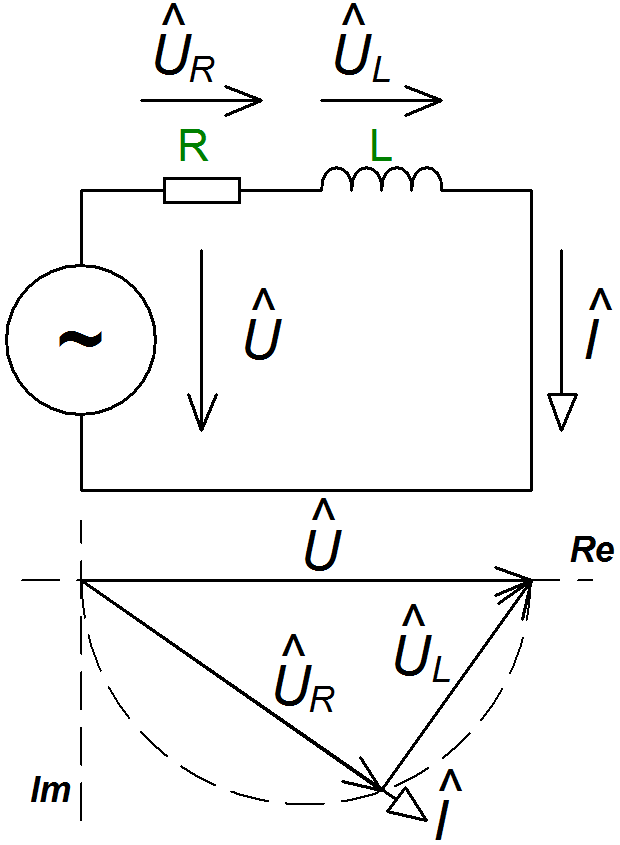
\includegraphics[scale=0.25]{obr01_RLobvod.png} &
			According to 2\textsuperscript{nd} Kirchhoff's law:
			$$\hat{U}=\hat{U}_R + \hat{U}_L = R\cdot\hat{I}+j\omega L\cdot\hat{I}$$
			Complex impedance:
			$$\hat{Z}=R+j\omega L$$
			\end{tabular}
		\end{center}
	\end{frame}
%------------------------------------------------------------------------------
%Impedance
%------------------------------------------------------------------------------
\section{\texorpdfstring{Excercises}{Excercises}}
%------------------------------------------------------------------------------
	\begin{frame}
    \frametitle{Behavior of Components at Harmonic Supply}
		\begin{enumerate}
			\setcounter{enumi}{0}
			\item Identify unknown components in the black-box through their response to a harmonic signal.
		\end{enumerate}
		
		\begin{center}
			\begin{tabular}{m{0.3\linewidth} m{0.6\linewidth}}
			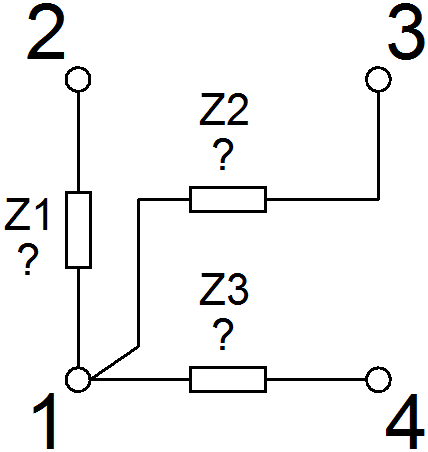
\includegraphics[scale=0.25]{obr02_identifikaceZ.png} &
			Voltage, current and frequency dependency for each component:
			$$\hat{U}=R \cdot \hat{I}$$
			$$\hat{U}=X_L \cdot \hat{I} = j\omega L \cdot\hat{I}$$
			$$\hat{U}=X_C \cdot \hat{I} = \frac{-j}{\omega C}\cdot\hat{I}$$
			\end{tabular}
		\end{center}
	\end{frame}
%------------------------------------------------------------------------------
	\begin{frame}
    \frametitle{Behavior of Components at Harmonic Supply}
		\begin{enumerate}
			\setcounter{enumi}{1}
			\item Create parallel connection of capacitor and resistor. Connect the circuit to the voltage source 4~V. Measure the current in each branch.
		\end{enumerate}
		
		\begin{center}
			\begin{tabular}{m{0.35\linewidth} m{0.55\linewidth}}
			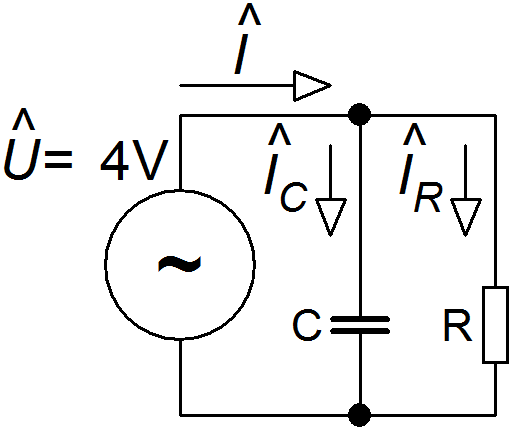
\includegraphics[scale=0.25]{obr03_RCobvod.png} &
			
			\begin{itemize}
				\item Do the current values respect 1\textsuperscript{st} Kirchhoffs law?
				\item Write the measured currents as a phasors (complex numbers).
				\item Draw a phasor diagram. Think about dissipation factor $D$, where is angle $\delta$?
			\end{itemize}
			\end{tabular}
		\end{center}
	\end{frame}
%------------------------------------------------------------------------------
	\begin{frame}
    \frametitle{Behavior of Components at Harmonic Supply}
		\begin{enumerate}
			\setcounter{enumi}{2}
			\item Create serial connection of capacitor and inductor. Connect the circuit to the voltage source 4~V. Measure the current and voltage drop over each component.
		\end{enumerate}
		
		\begin{center}
			\begin{tabular}{m{0.4\linewidth} m{0.5\linewidth}}
			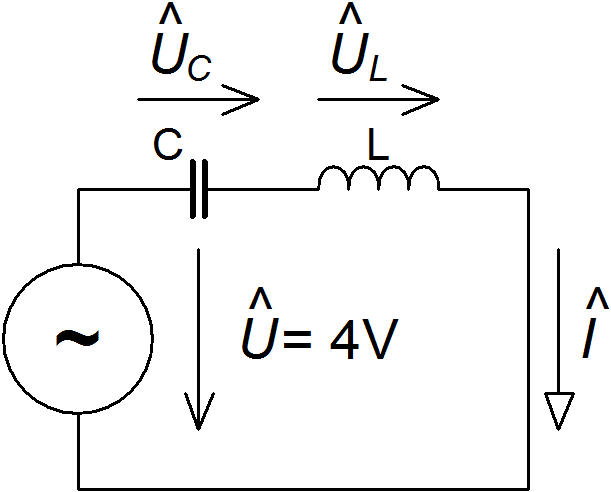
\includegraphics[scale=0.25]{obr04_LCobvod.png} &
			
			\begin{itemize}
				\item Do the voltage values respect 2\textsuperscript{nd} Kirchhoffs law?
				\item Write the measured voltages as a phasors (complex numbers).
				\item Draw a phasor diagram. Think about qulity factor $Q$. How can you determine it?
			\end{itemize}
			\end{tabular}
		\end{center}
	\end{frame}
%------------------------------------------------------------------------------
\end{document}